Ein wichtiger Teil für die Arbeit mit der Hololens sind die Grafiken mit denen man \\ interagiert. Ohne diese ist ein AR Headset nicht verwendbar.\\
\subsection{Limits der Hololens2}\label{subsec:Limits der Hololens2}

Auf der Hololens gibt es limits von Objekten und deren Anzahl an Dreiecken.
Diese Limits gibt es aufgrund der Prozessorleistung des eingebauten Prozessors und der Kühlungskapazität von dem eingebautem Kühler.
Die Temperaturlimits sind nicht nur wegen dem schutz der Hardware sondern auch dem Tragekomfor bedingt.\\
Microsoft schlägt für die Objekte in einer szene ein Dreieck limit an. Diese Limits sind für bis zu drei Objekte in der Szene, bei bis zu 100.000\autocite{optimize_3d} Dreiecke pro Objekt.\\
Diese Limits sind nur Empfehlungen die für den Test wichtig sind da man an dieser Anzahl sehen kann inwieweit man diese überschritten hat.
Durch Tests kann abgeleitet werden inwiefern man sich an die vorgeschlagenen Limits halten muss, bevor man an die Limits des Prozessors kommt.\\
Somit kann man schon bei der erstellung einer Szene schon einschätzen ob die Leistung beeinflusst werden würde oder ob man noch im einem akzeptablen Bereich liegt.

%¹microsoft seite mit limit werten
%Die von microsoft gegebenen limits¹ die für die anfänglichen test wichtig sind 
%lagen bei weniger als 100.000 dreiecke pro objekt 
%bei drei objekten in der szene. 

%Da das aber empfehlungen waren haben wir ein objekt mit vielen polygonen genommen,
%die diese anzahl deutlich überschreiten.
%durch diese tests kann man dann ableiten ob eine modelierte szene auch performant 
%auf dem endgerät laufen wird, oder unerwünschte
%performance veringerungen entstehen könnten. mit dieser information kann man 
%masnahmen einleiten die die performance so hoch wie 
%möglich hält.

    \newpage

\subsection{Testobjekte}\label{subsec:Testobjekte}


Für die Tests sind zwei Objekte gewählt die jeweils über und unter dem vorgeschlagenem Limit \autocite{optimize_3d} sind.
Das kleinere Objekt ist ein Affenkopf \autocite{Blender_primitives} das standartmäsig mit dem Programm Blender \autocite{Blender} mitgeliefert kommt.
Das Größere Objekt ist der Fraktal Würfel Mengersponge der in Blender \autocite{Blender} mit einem Plugin \autocite{Blender_Extra_Objects} generiert wurde.\\
Beide objekte wurden jeweils als fbx Datei exportiert.
Die Dateigröße des Affenkopfs ist 47KB und die des Fraktals 9838KB.
Diese Dateigrößen kommen von den verschiedenen Dreieck Anzahlen. Die Anzahl bei dem Fraktal ist 672.768 Dreiecke und bei dem Affenkopf 968 Dreiecke.\\
 Durch diese Testobjekte soll die Leistung der Hololens einschätzbar werden.
\begin{figure}[ht!]
    \center
    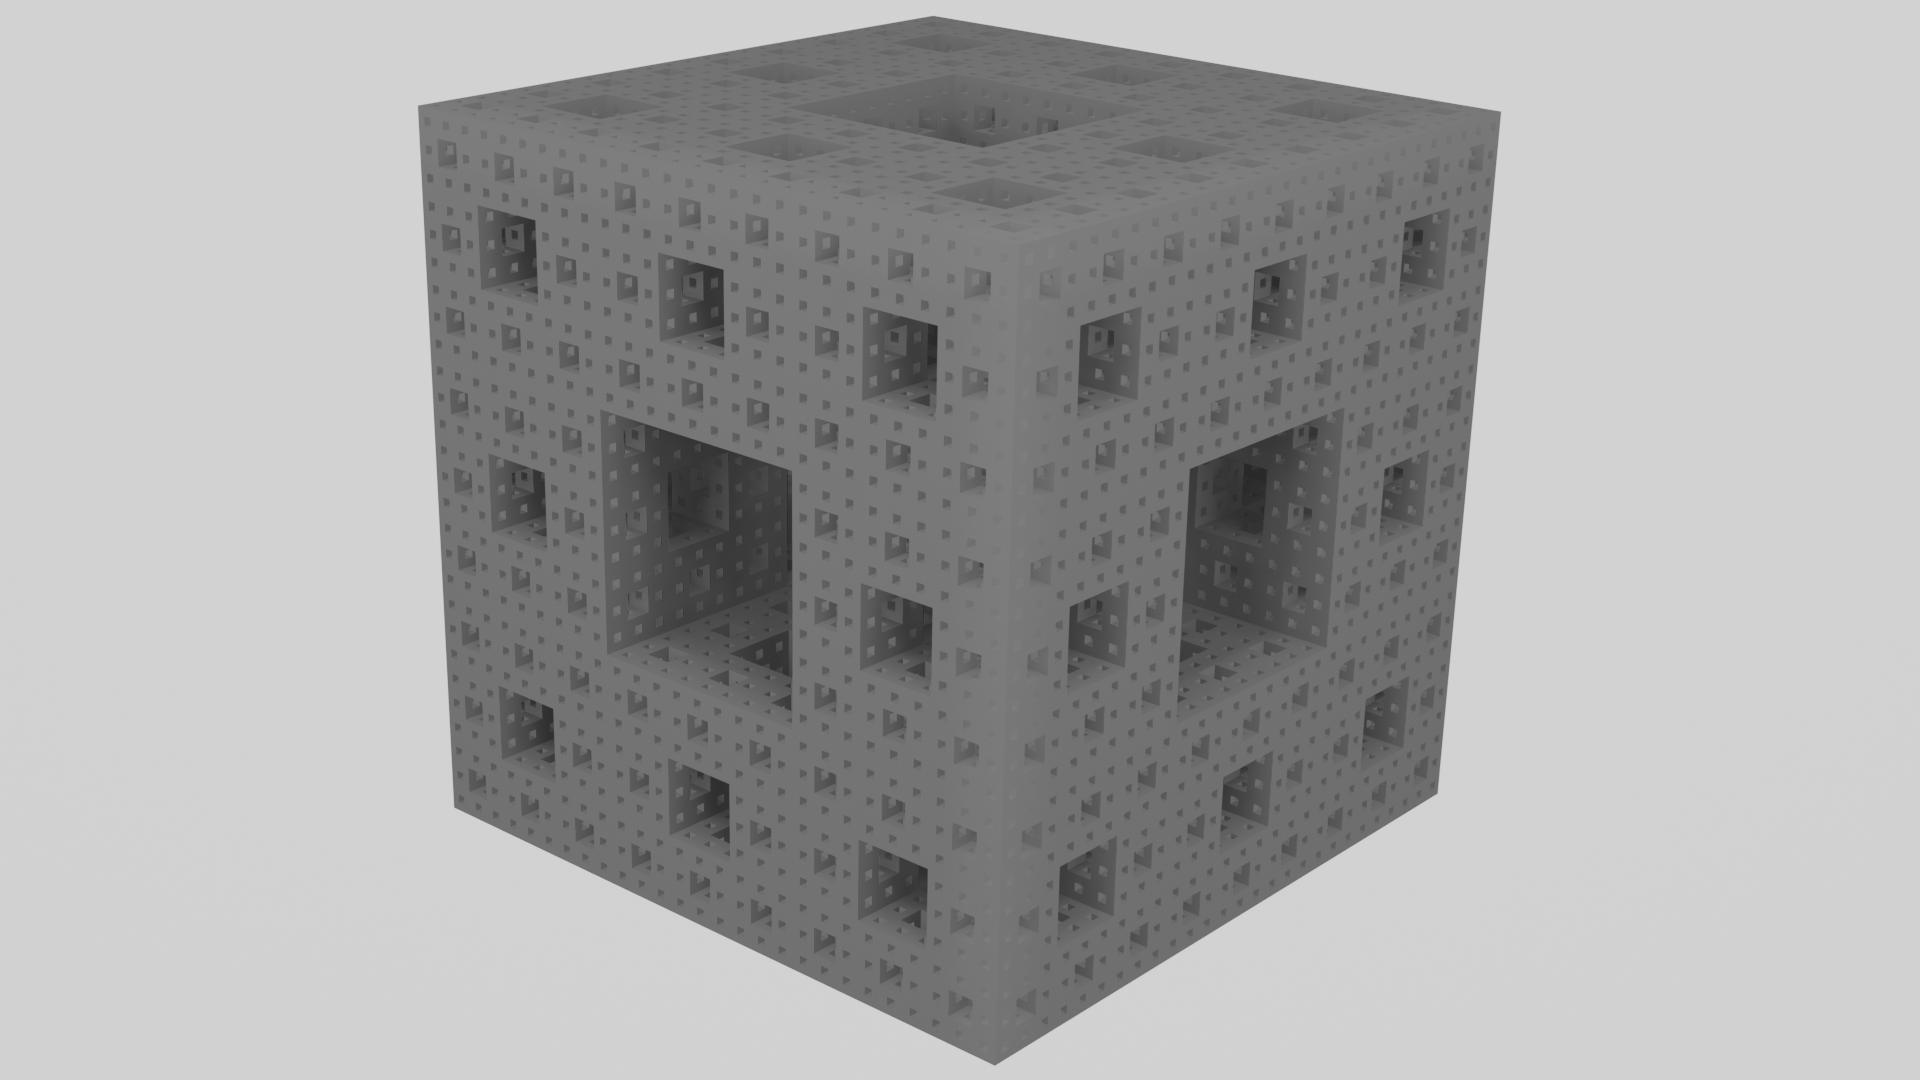
\includegraphics[trim={13cm 0 13cm 0},clip,width={0.5\textwidth}]{../assets/img/menger_sponge.png}
    \caption{Mengersponge \autocite{Blender_Extra_Objects}}
    \label{fig:Mengersponge}
\end{figure}
\begin{figure}[ht!]
    \center
    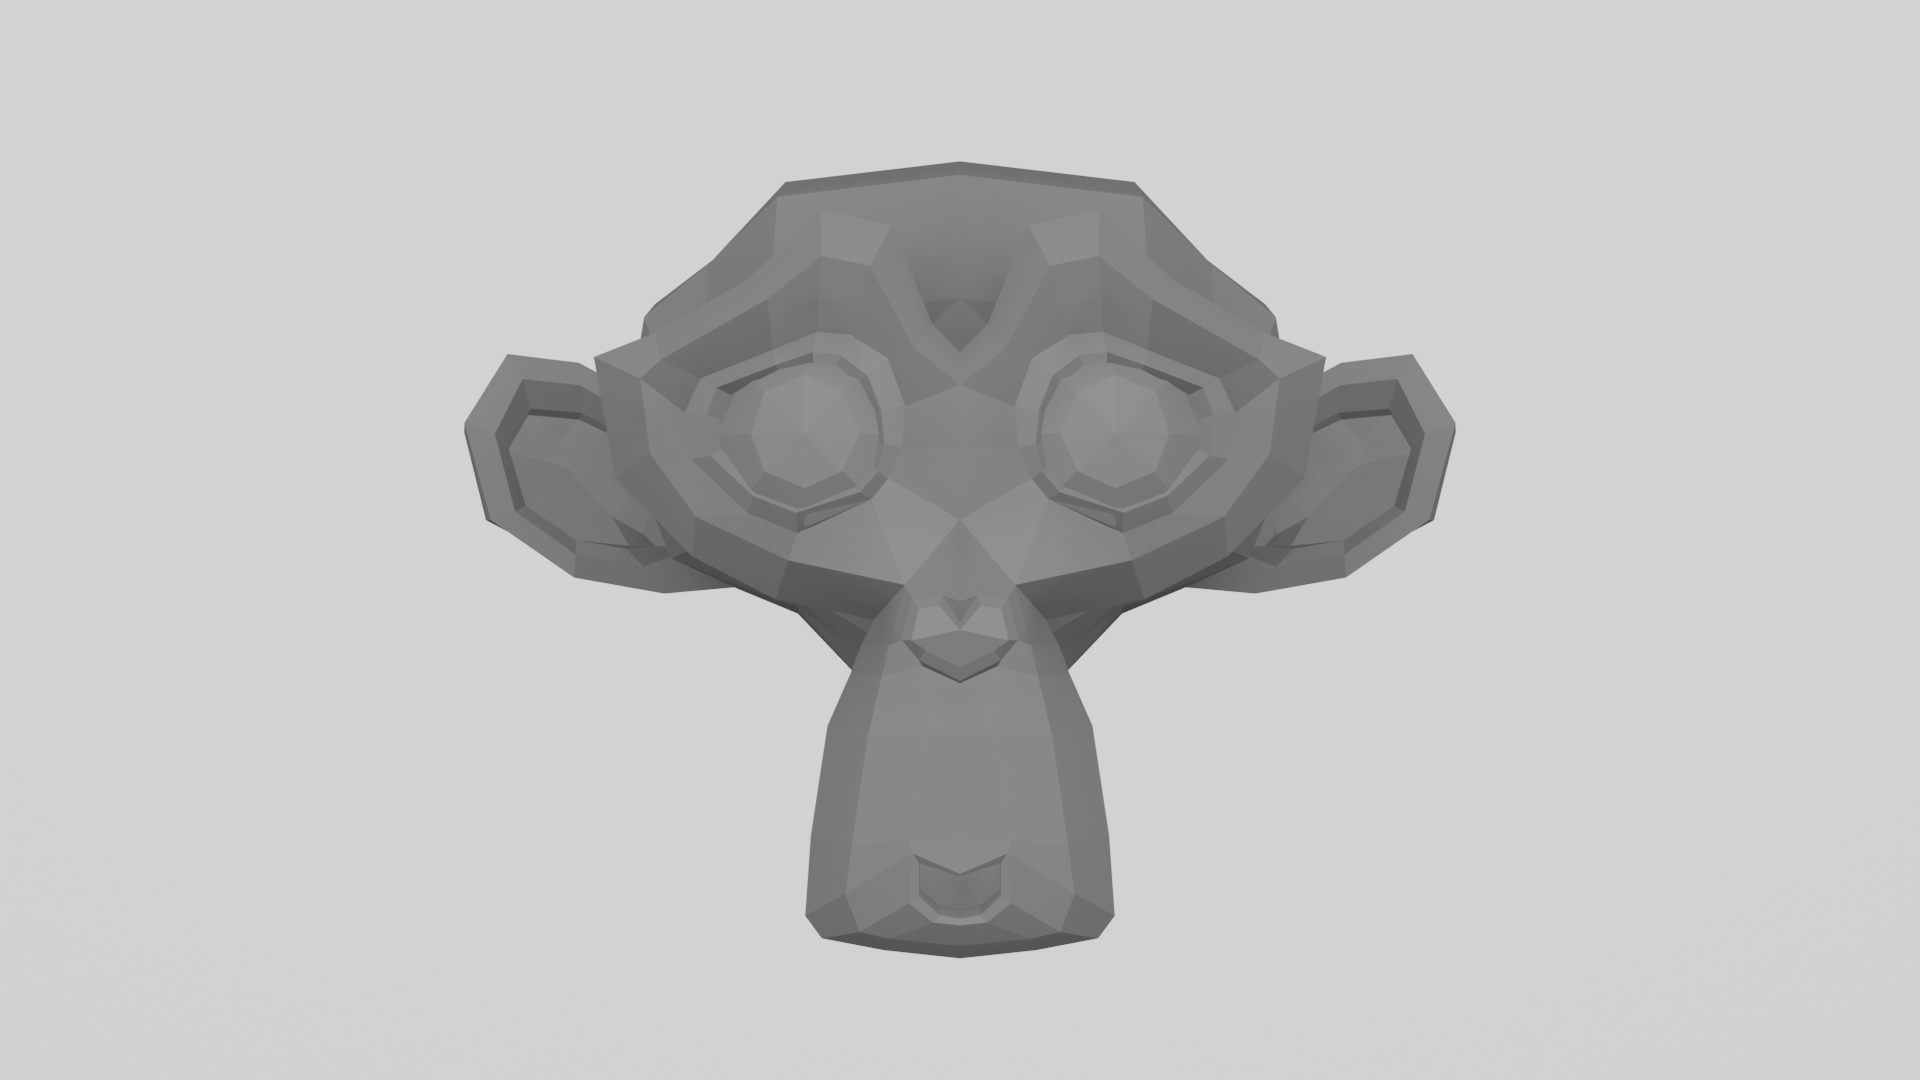
\includegraphics[trim={14cm 3cm 14cm 4cm},clip,width={0.5\textwidth}]{../assets/img/monkey.png}
    \caption{Monkey \autocite{Blender_primitives}}
    \label{fig:Menonkey}
\end{figure}


%Als testobjekt wurde ein mengersponge fraktal und ein default affenkopf aus blender jeweils als fbx datei exportiert.
%die größe der datei des fraktals begab sich auf 9838KB und die des affenkopfs auf 47KB. die dreiekanzahl sind für das fraktal
%672.768 und für den affenkopf 968. diese objekte sind gewählt da sie auf zwei verschiedenen enden des limits sind.
%der affenkopf ist weniger als das limit und als test innerhalb der limitation und das fraktal als element weit oberhalb der limit grenze
%die auf der microsoft¹ seite zu finden ist.
    \newpage

\subsection{Test verfahren}\label{subsec:Test verfahren}
Auf der Hololens exsistiert ein Programm das 3d Objekte anzeigen kann.
Dieses Programm wird als erster Test genutzt.
Bei diesem Test wird getestet ob das Objekt in diesem Programm geladen werden kann.
Der zweite Test ist das Objekt wird in ein Unity projekt importiert und ausführt.
Das Unity pojekt wird dann auf der Hololens ausgeführt und getestet.
Dann wird geschaut ob ein Unterschied besteht.\\
Die wichtigsten Datenpunkte für diese Tests sind die fps, Dreieckanzahl, und ob das Objekt angezeigt werden kann.
Durch die Ergebnisse der Tests wird dann klar wo in etwa die Limits liegen und ob diese über oder unter dem vorgeschlagenen Limits \autocite{optimize_3d} liegen die von Microsoft vorgeschlagen wurden.


%erst wird getestet ob die objekte in dem vorinstallierten 3d viewer ladbar sind.
%nach diesen test werden die objekte in dem unity projekt importert und auf der hololens ausgeführt.
%die wichtigsten datenpunkte sind die fps, polygon anzahl und ob das objekt direkt angesegen wird oder nicht.
%nach diesen tests sind die limits für ein problemloses laufen des programms klar und man kann sehen in wie weit die limits, 
%die von microsoft vorgeschlagen sind eingegalten werden müssen.

\subsection{Test durchführung}\label{subsec:Test durchführung}
In der vorinstallierten Software wird versucht, jeweils das Objekt zu laden.
Der Affenkopf wurde ohne weitere probleme geladen.
Bei dem Fraktal hat das Programm eine Fehlermeldung gegeben, dass es das Objekt nicht laden konnte.\\
Da nur das Fraktal ein Problem gegeben hat wurde es als erstes für den Test mit der unity game engine \autocite{unity} gewählt.
Nach dem importieren und hochladen auf die Hololens wird das Programm gestartet.\\
Während der Laufzeit des Programms wurde festgestellt dass die fps die von der Hololens anzeigt wird und und welche man wirklich sieht anders sind.\\
Man hat gesehen dass das Programm in einer anderen fps berechnet wird als wie sie angezeigt wird.
Die fps die von der Hololens berichtet wurden haben sich auf drei verschiedene Szenarien verteilt.
Wenn man das Objekt direkt im Anzeigebereich sah, waren die fps die berichtet wurden auf 16 fps runter gegangen.
Wenn in die Richtung des Objeks geschaut wurde ohne dass es in dem Anzeigebereich zu sehen war wahren die fps höher.
Die fps waren am höchsten wenn das objekt 180 grad hinter der Hololens war.\\
Durch verschiedenste setup Probleme und am ende fehlende Zeit war es uns nicht möglich genaue Daten für diese fps tests zu bekommen.

\subsection{Verbesserungsmethoden}\label{subsec:Verbesserungsmethoden}

Es gibt Möglichkeiten die Objekte in voraus zu optimieren.
Einige Methoden sind schon auf der seite von Microsoft \autocite{best_practices} beschrieben.\\
Texturen können kleiner gemacht werden und als eine Textur in dem Propjekt importiert werden.
Bei Objekten mit einem Inneleben das nicht gesehen wird kann man die nicht sichtbare Geometrie einfach entfernen.
Eine weitere Optimisierungsmöglichkeit ist das die Dreieckanzahl soweit wie möglich zu verringern so dass nicht zu große Objekte geladen werden müssen.
Objekte die nicht voneinander getrennt werden müssen können zu einem Objekt zusammen gefügt werden.

%²microsoft seite vorschläge für optimisierung
%durch einfaches importieren des fraktals in das unity projekt konnte es angezeigt werden obwohl es sichtbare performance probleme
%generiert hat. 
%Durch externe optimisierungs optionen² kann die performance durchaus verbessert werden.
%man kann texturen kleiner² machen und mehrere² als eine textur importiern.
%Bei objekten die ein innenleben² haben oder objekte/flächen² die nicht gesehen werden, kann man diese einfach löschen so dass 
%die nicht erst in der laufzeit ignoriert werden müssen. eine weitere optimisierung ist dass man objekte die nicht voneinander
%getrennt werden einfach als ein objekt zusammengefügt² werden.

\subsection{Zukünftige verbesserungsmöglichkeiten}\label{subsec:Zukünftige verbesserungsmöglichkeiten}

In der Zukunft gib es verschiedenste möglichkeiten die Performance zu verbessern.
Mit einem Stand Pc und einer kabelosen Verbindung zu einem AR Gerät kann die Leistung von dem Headset abgekoppelt werden.
Damit kann die Leistung von dem PC hoch genug für die Applikation gewählt werden.\\
Es ist mit einem Dienst für Anwendungsstreaming auch möglich die Prozessorleistung zu limitieren die das Headset leisten muss.
Wenn die Streamingmethoden nicht möglich sind können die zukünftige AR Headsets mit stärkeren mobilen Prozessoren ausgerüstet werden. Mit einem stärkeren Prozessor sind die limits viel höher, dies ist aber oft zur jeweiligen Zeit nicht möglich.
%Es gibt einige möglichkeiten die performance für ar in der zukunft zu verbessern.
%durch ein desktop pc und kabelose verbinung kann man die performance verbessern und den komfort, da nur die anzeige seite auf
%dem headset unterstütst werden muss. falls keine möglichkeit für einen eigenen pc für streaming vorhanden ist kann auch ein online
%service mit der computing performance möglich sein. dadurch braucht das headset nur kleine leistung um das video streaming zu 
%unterstützen. durch verbesserungen in der mobilen chip technologien kann das headset in der zukunft kleiner, leichter und zur gleichen
%zeit performanter werden. dadurch würden die heutigen limitationen dann weiter zurückgeschoben werden.

